\documentclass[epsfig,10pt,fullpage]{article}

\newcommand{\LabNum}{7}
\newcommand{\CommonDocsPath}{../../../common/docs}
\addtolength{\textwidth}{1.5in}
\addtolength{\oddsidemargin}{-0.75in}
\addtolength{\topmargin}{-0.75in}
\addtolength{\textheight}{1.5in}
\addtolength{\evensidemargin}{0.75in}
\setlength\parindent{0pt}
\raggedbottom

\usepackage{ae,aecompl}
\usepackage{epsfig,float,times}
\usepackage[hypcap]{caption}
\usepackage[pdftex, colorlinks]{hyperref}
\usepackage{graphicx}
\usepackage[usenames, dvipsnames]{color}
\usepackage{rotating}
\usepackage{tikz}
\usetikzlibrary{automata,positioning}
\usepackage{placeins}

\widowpenalty 10000
\clubpenalty 10000

\newcommand{\red}[1]{{\color{red}\sf{#1}}}
\newcommand{\green}[1]{{\color{green}\sf{#1}}}
\newcommand{\blue}[1]{{\color{blue}\sf{#1}}}
\definecolor{PineGreen}{rgb}{0.0, 0.47, 0.44}
\definecolor{ForestGreen}{rgb}{0.13, 0.55, 0.13}
\definecolor{Brown}{rgb}{0.59, 0.29, 0.0}

\newcommand{\UPDatePublished}{Oct 2021}
\newcommand{\versnum}{21.1} %version number quartus/AMP
\newcommand{\quartusname}{Quartus\textsuperscript{\textregistered} Prime}	
\newcommand{\UPTextBar}{For \quartusname{} \versnum{}}
\newcommand{\thisyear}{2021 } %for copyright
\newcommand{\company}{FPGAcademy.org}
\newcommand{\longteamname}{FPGAcademy.org}
\newcommand{\teamname}{FPGAcademy}
\newcommand{\website}{FPGAcademy.org}

\newcommand{\productAcronym}{AMP}
\newcommand{\productNameShort}{Monitor Program}

\newcommand{\productNameMedTM}{A Monitor Program}
\newcommand{\productNameMed}{A Monitor Program}

%\newcommand{\headerLogoFilePath}[1]{#1/FPGAcademy.png}

% listings is a package that supports encapsulating source code in LaTeX conveniently
\usepackage{listings}

\def\expandparam\lstinputlisting[#1]#2{\edef\tmp{\noexpand\lstinputlisting[#1]{#2}}\tmp}

%%%%%%%%%%%%%%%%%%%% Source Code Formatting %%%%%%%%%%%%%%%%%%%%
\definecolor{globalCommentColour}{rgb}{0.588,0.588,0.588}

%%%%%%%%%%%%%%%%%%%%%%%%%%%%%%%%%%%%%%%%%%%%%%%%%%%%
% Defining language style
% NiosII ASM
\lstdefinelanguage[NiosII]{Assembler} {
  morekeywords={add, addi, and, andhi, andi, beq, bge, bgeu, bgt, bgtu, ble,  bleu, blt, bltu, bne, br, break,
  bret, call, callr, cmpeq, cmpeqi, cmpge, cmpgei, cmpgeu, cmpgeui, cmpgt, cmpgti, cmpgtu, cmpgtui, cmple,
  cmplei, cmpleu, cmpleui, cmplt, cmplti, cmpltu, cmpltui, cmpne, cmpnei, custom, div, divu, eret, flushd,
  flushda, flushi, flushp, initd, initda, initi, jmp, jmpi, ldb, ldbio, ldbu, ldbuio, ldh, ldhio, ldhu, ldhuio,
  ldw, ldwio, mov, movhi, movi, movia, movui, mul, muli, mulxss, mulxsu, mulxuu, nextpc, nop, nor, or, orhi, ori,
  rdctl, rdprs, ret, rol, roli, ror, sll, slli, sra, srai, srl, srli, stb, stbio, sth, sthio, stw, stwio,
  sub, subi, sync, trap, wrctl, wrtcl, wrprs, xor, xori, xorhi, xori},
  morekeywords=[2]{.abort, .ABORT, .align, .app-file, .ascii, .asciz, .balign, .byte, .comm, .data, .def,
  .desc, .dim, .double, .eject, .else, .end, .endef, .endif, .equ, .equiv, .err, .extern, .file, .fill, .float,
  .global, .globl, .hword, .ident, .if, .include, .int, .irp, .irpc, .lcomm, .lflags, .line, .linkonce, .ln,
  .list, .long, .macro, .mri, .nolist, .octa, .org, .p2align, .psize, .quad, .rept, .sbttl, .scl, .section,
  .set, .short, .single, .size, .sleb128, .skip, .space, .stadb, .stabn, .stabs, .string, .symver, .tag,
  .text, .title, .type, .val, .uleb128, .word},
  morekeywords=[3]{et, bt, gp, sp, fp, ea, sstatus, ra, pc, status, estatus, bstatus, ienable, ipending, cpuid,
  exception, pteaddr, tlbacc, tlbmisc, eccinj, badaddr, config, mpubase, mpuacc},
  sensitive=t,
  alsoletter=.,
  morestring=[b]",
  morecomment=[s]{/*}{*/},
  morecomment=[l]\#,
}[keywords,comments,strings]
   
%% NOTE: morekeywords=[2] are GNU directives.
   
\definecolor{niosInstructionColour}{rgb}{0.000,0.608,0.000}
\definecolor{niosDirectiveColour}{rgb}{0.000,0.000,0.902}
\definecolor{niosSpecialRegColour}{rgb}{0.000,0.000,0.000}
\definecolor{niosStringColour}{rgb}{0.808,0.482,0.000}
   
%% NOTE: To make bold use: =\bfseries\color{<colour>}
\lstdefinestyle{defaultNiosStyle} {
  language=[NiosII]{Assembler},
  stringstyle=\color{niosStringColour},
  keywordstyle=\color{niosInstructionColour},
  keywordstyle=[2]\color{niosDirectiveColour},
  keywordstyle=[3]\itshape\color{niosSpecialRegColour}
}
%%%%%%%%%%%%%%%%%%%%%%%%%%%%%%%%%%%%%%%%%%%%%%%%%%%%

%%%%%%%%%%%%%%%%%%%%%%%%%%%%%%%%%%%%%%%%%%%%%%%%%%%%
% Defining language style
% ArmA9 ASM
\lstdefinelanguage[ArmA9]{Assembler} {
  morekeywords={ADC, ADD, ADDS, AND, ANDS, B, BAL, BEQ, BGE, BGT, BL, BLT, BIC, BKPT, BLX, BNE, BX, CDP, CLZ, CMN, CMP, EOR,
  EORS, LDC, LDM, LDR, LDRB, LDRBT, LDRH, LDRSB, LDRSH, LDRT, LSL, MCR, MLA, MOV, MOVW, MOVT, MRC, MRS, MSR, MUL, MVN, ORR, PLD,
  ROR, RSB, RSC, SBC, SMLAL, SMULL, STC, STM, STR, STRB, STRBT, STRH, STRT, SUB, SUBS, SWI, SWP, SWPB, TEQ, UMLAL,
  PUSH, POP, MOVS, RORS, LSR},
  morekeywords=[2]{.abort, .ABORT, .align, .app-file, .ascii, .asciz, .balign, .byte, .comm, .data, .def,
  .desc, .dim, .double, .eject, .else, .end, .endef, .endif, .equ, .equiv, .err, .extern, .file, .fill, .float,
  .global, .globl, .hword, .ident, .if, .include, .int, .irp, .irpc, .lcomm, .lflags, .line, .linkonce, .ln,
  .list, .long, .macro, .mri, .nolist, .octa, .org, .p2align, .psize, .quad, .rept, .sbttl, .scl, .section,
  .set, .short, .single, .size, .sleb128, .skip, .space, .stadb, .stabn, .stabs, .string, .symver, .tag,
  .text, .title, .type, .val, .vectors, .uleb128, .word},
  morekeywords=[3]{SP, PC, MIDR, CTR, TCMTR, TLBTR, MPIDR, ID_PFR0, ID_PFR1, ID_DFR0, ID_MMFR0, ID_MMFR1, ID_MMFR2,
  ID_MMFR3, ID_ISAR0, ID_ISAR1, ID_ISAR2, ID_ISAR3, ID_ISAR4, CCSIDR, CLIDR, AIDR, CSSELR, TTBR0, TTRB1, TTBR2, DACR,
  DFSR, IFSR, ADFSR, AIFSR, DFAAR, IFAR, ICIALLUIS, BPIALLIS, PAR, ICIALLU, ICIMVAU, BPIALL, DCIMVAC, DCISW, V2PCWPR,
  DCCVAC, DCCSW, DDIMVAC, DCISW, TLBALLIS, TLBIMVAIS, TLBIASIDIS, TLBIMVAAIS, TLBIALL, TLBIMVA, TLBIASID, TLBIMVAA,
  PMCR, PMCNTENSET, PMCNTENCLR, PMOVSR, PMSWINC, PMSELR, PMXEVTYPER, PMXEVCNTR, PMUSERENR, PMINTENSET, PMINTENCLR,
  PRRR, NRRR, PLEIDR, PLEASR, PLEFSR, PLEUAR, PLEPCR, VBAR, MVBAR, ISR, FCSEIDR, CONTEXTIDR, TPIDRURW, TPIDRURO, TPIDRPRW},
  sensitive=f,
  alsoletter=.,
  morestring=[b]",
  morecomment=[s]{/*}{*/},
  morecomment=[l]{//},
}[keywords,comments,strings]
   
%% NOTE: morekeywords=[2] are GNU directives.
   
\definecolor{armInstructionColour}{rgb}{0.000,0.608,0.000}
\definecolor{armDirectiveColour}{rgb}{0.000,0.000,0.902}
\definecolor{armSpecialRegColour}{rgb}{0.000,0.000,0.000}
\definecolor{armStringColour}{rgb}{0.808,0.482,0.000}
   
\lstdefinestyle{defaultArmStyle} {
  language=[ArmA9]{Assembler},
  stringstyle=\color{armStringColour},
  keywordstyle=\color{armInstructionColour},
  keywordstyle=[2]\color{armDirectiveColour},
  keywordstyle=[3]\itshape\color{armSpecialRegColour}
}
%%%%%%%%%%%%%%%%%%%%%%%%%%%%%%%%%%%%%%%%%%%%%%%%%%%%

%%%%%%%%%%%%%%%%%%%%%%%%%%%%%%%%%%%%%%%%%%%%%%%%%%%%
% Defining language style
% FPGAcademy ASM
\lstdefinelanguage{ASM}{
  morekeywords = [1]{mv, mvt, mvne, mvcc, add, sub, st, ld, and, b, bne, beq, bcc, bcs},
  morekeywords = [2]{word, define},
  keywordstyle = [1]\color{ForestGreen},
  keywordstyle = [2]\color{blue},
  sensitive = true,
  morecomment = [l]{//},
}

\lstset{
  language = ASM,
  basicstyle=\small\color{black}\ttfamily,
  commentstyle=\small\color{Brown}\itshape\ttfamily,
  showstringspaces=false,
  frame=none, %lines % boxed listings
  breaklines=true,
  breakatwhitespace=true,
  tabsize=3
}
%%%%%%%%%%%%%%%%%%%%%%%%%%%%%%%%%%%%%%%%%%%%%%%%%%%%

%%%%%%%%%%%%%%%%%%%%%%%%%%%%%%%%%%%%%%%%%%%%%%%%%%%%
% Defining language style
% Java
\definecolor{javaStringColour}{rgb}{0.808,0.482,0}
%%%%%%%%%%%%%%%%%%%%%%%%%%%%%%%%%%%%%%%%%%%%%%%%%%%%

%%%%%%%%%%%%%%%%%%%%%%%%%%%%%%%%%%%%%%%%%%%%%%%%%%%%
% Defining language style
% C
\definecolor{CStringColour}{rgb}{0.808,0.482,0}

\lstset{
  language = C,
  basicstyle=\small\color{black}\ttfamily, 
  commentstyle=\small\color{PineGreen}\itshape\ttfamily,
  keywordstyle=\small\color{blue}\bfseries\ttfamily,
  showstringspaces=false,
  frame=none, %lines % boxed listings
  breaklines=true,
  breakatwhitespace=true,
  tabsize=3
}
%%%%%%%%%%%%%%%%%%%%%%%%%%%%%%%%%%%%%%%%%%%%%%%%%%%%

%%%%%%%%%%%%%%%%%%%%%%%%%%%%%%%%%%%%%%%%%%%%%%%%%%%%
% Defining language style
% Verilog
\definecolor{verilogCommentColour}{rgb}{0.000,0.502,0.000}

\lstdefinestyle{defaultVerilogStyle} {
  language={Verilog},
  keywordstyle=\color{blue},
  commentstyle=\color{verilogCommentColour}
}
%%%%%%%%%%%%%%%%%%%%%%%%%%%%%%%%%%%%%%%%%%%%%%%%%%%%

%%%%%%%%%%%%%%%%%%%%%%%%%%%%%%%%%%%%%%%%%%%%%%%%%%%%
% Defining language style
% VHDL
\lstdefinestyle{defaultVHDLStyle} {
  language={VHDL},
  keywordstyle=\color{blue},
  commentstyle=\color{verilogCommentColour}
}
%%%%%%%%%%%%%%%%%%%%%%%%%%%%%%%%%%%%%%%%%%%%%%%%%%%%

%%%%%%%%%%%%%%%%%%%%%%%%%%%%%%%%%%%%%%%%%%%%%%%%%%%%
% Defining language style
% LaTeX
\lstdefinelanguage[LocalLaTeX]{TeX}[LaTeX]{TeX}{moretexcs={bf, it, sf, lstset},}

\lstdefinestyle{defaultLocalLatexStyle} {
  language=[LocalLatex]{TeX},
  keywordstyle=\color{blue}\bfseries,
  keywordstyle=[2]\color{blue},
  keywordstyle=[3]\color{blue}\bfseries
}
%%%%%%%%%%%%%%%%%%%%%%%%%%%%%%%%%%%%%%%%%%%%%%%%%%%%

%%%%%%%%%%%%%%%%%%%%%%%%%%%%%%%%%%%%%%%%%%%%%%%%%%%%
% Defining language style
% Default
\lstset{
  basicstyle=\small\color{black}\ttfamily,
  commentstyle=\small\color{globalCommentColour}\itshape\ttfamily,
  keywordstyle=\small\color{blue}\bfseries\ttfamily,
  showstringspaces=false,
  frame=none, %lines % boxed listings
  breaklines=true,
  breakatwhitespace=true,
  tabsize=3
}
%%%%%%%%%%%%%%%%%%%%%%%%%%%%%%%%%%%%%%%%%%%%%%%%%%%%


\hypersetup{
  pdftitle={Digital Logic Lab Exercise \LabNum},
  linkcolor=blue,
  hyperindex=true,
  pdfauthor={FPGAcademy.org},
  pdfkeywords={FPGAcademy.org, FPGAcademy, Lab, Exercise, Digital Logic},
  bookmarks,
  bookmarksopen=false,
  filecolor=blue,
  pdfstartview={FitH},
  urlcolor=blue,
  plainpages=false,
  pdfpagelabels=true,
  linkbordercolor={1 1 1} %no color for link border
}



\begin{document}

\centerline{\huge Digital Logic}
~\\
\centerline{\huge Laboratory Exercise \LabNum}
~\\
\centerline{\large Finite State Machines}
~\\

\noindent
This is an exercise in using finite state machines.
~\\

\section*{Part I}
\addcontentsline{toc}{1}{Part I}
We wish to implement a finite state machine (FSM) that recognizes two specific sequences 
of applied input symbols, namely four consecutive 1s or four consecutive 0s. There is an 
input $w$ and an output $z$. Whenever $w = 1$
or $w = 0$ for four consecutive clock pulses the value of $z$ has to be 1; 
otherwise, $z = 0$. Overlapping sequences
are allowed, so that if $w = 1$ for five consecutive clock pulses the output $z$
will be equal to 1 after the fourth and
fifth pulses. Figure~\ref{fig:sequence_diagram} illustrates the required relationship between $w$ and $z$.

\begin{figure}[H]
\centerline{
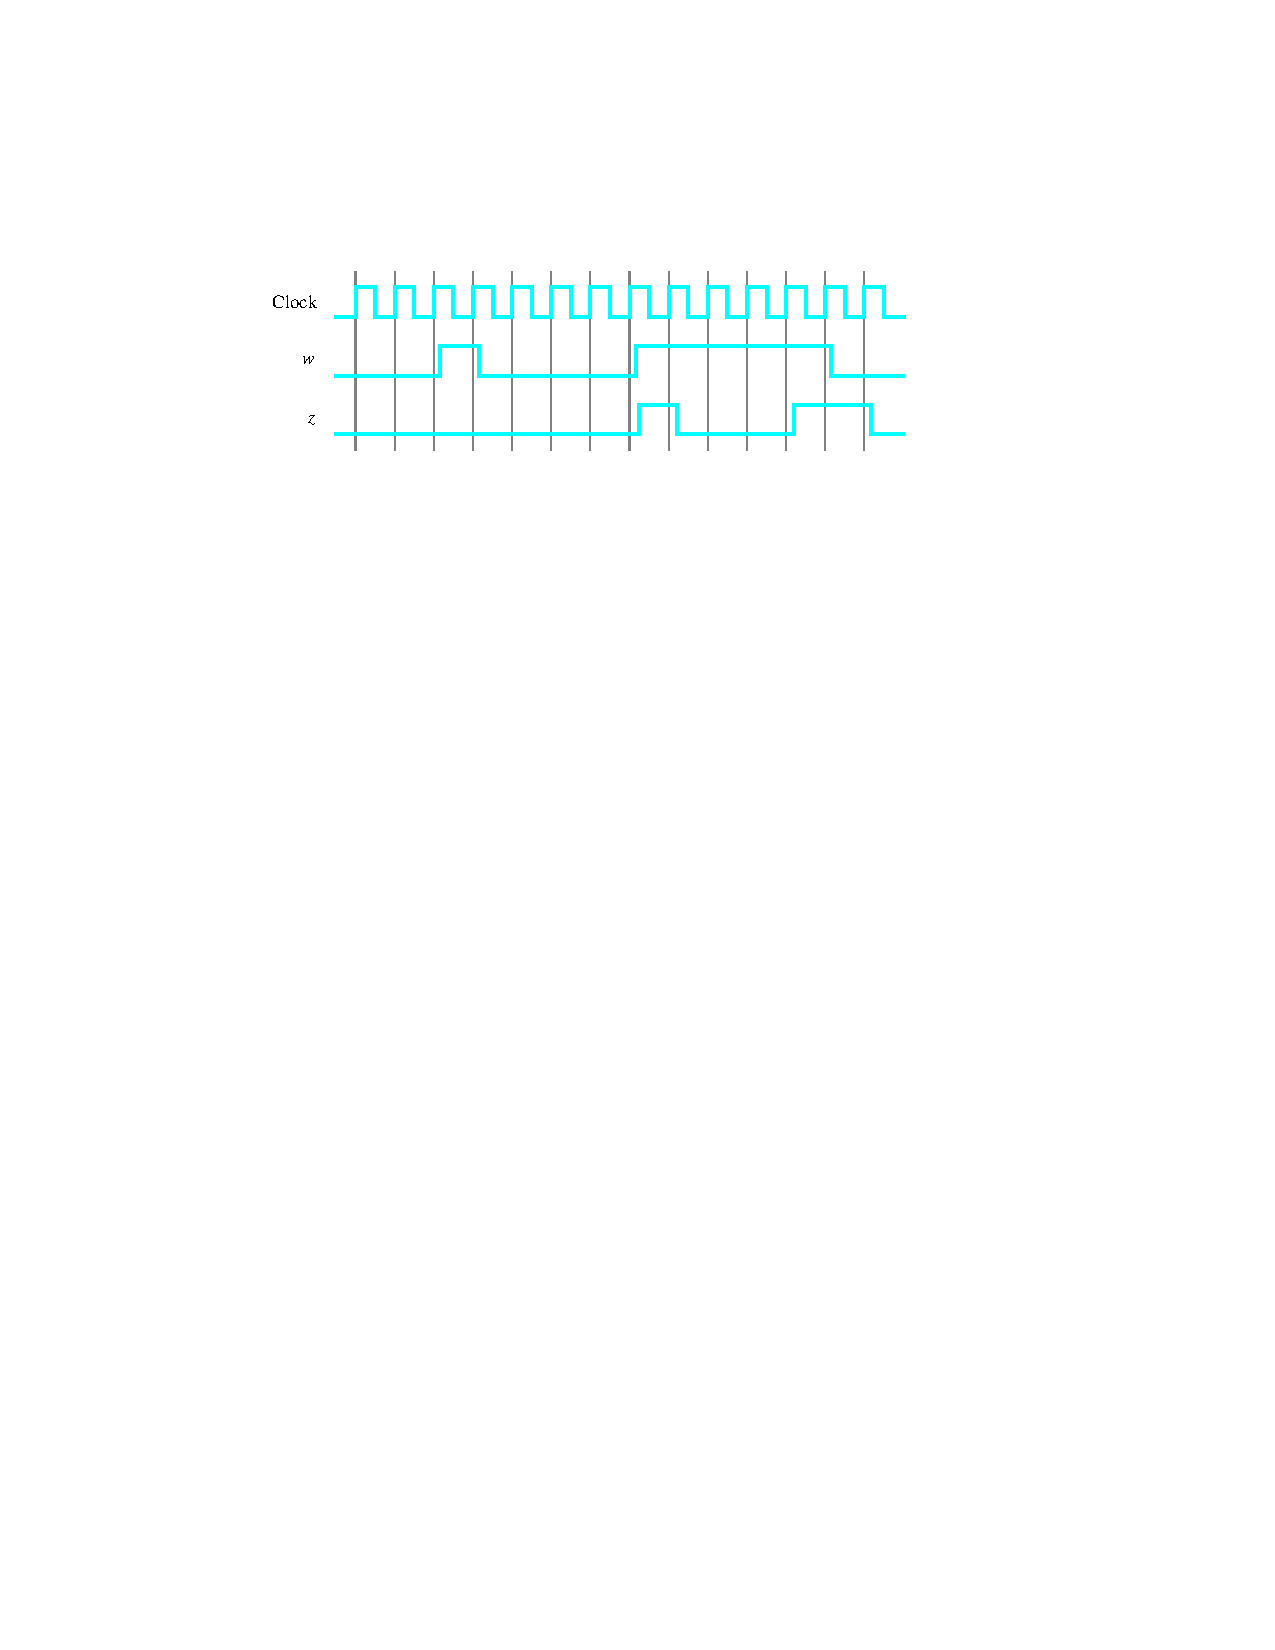
\includegraphics{figures/figure1.pdf}}
\caption{Required timing for the output $z$.}
\label{fig:sequence_diagram}
\end{figure}

A state diagram for this FSM is shown in Figure~\ref{fig:state_diagram}. For this part you are to manually
derive an FSM circuit that implements this state diagram, including the logic expressions
that feed each of the state flip-flops. To
implement the FSM use nine state flip-flops called $y_8, \ldots, y_0$ and the 
one-hot state assignment given in Table~\ref{tab:state_assignment}.

\begin{figure}[H]
\centerline{
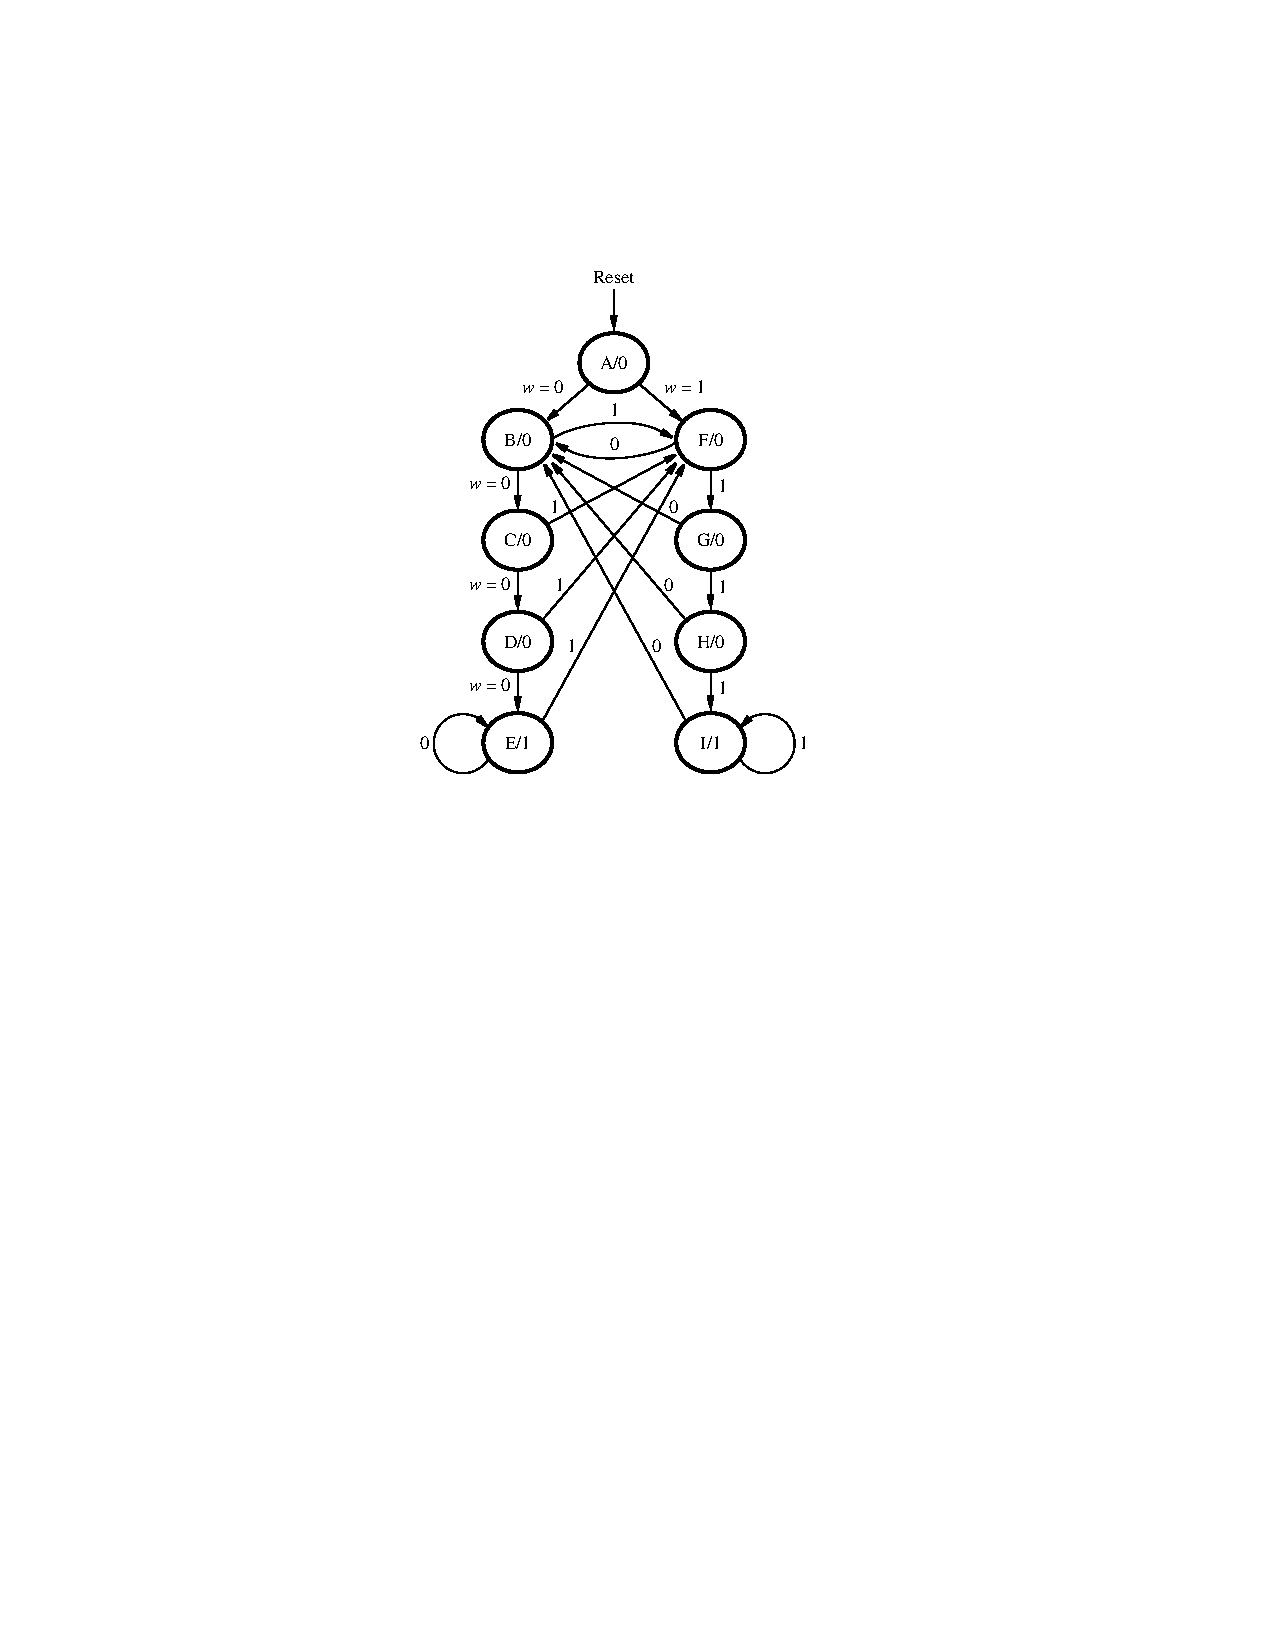
\includegraphics{figures/figure2.pdf}}
\caption{A state diagram for the FSM.}
\label{fig:state_diagram}
\end{figure}

\begin{table}[H]
\begin{center}
\begin{tabular}{c|c}
~ & State Code \\ 
Name & $y_8 y_7 y_6 y_5 y_4 y_3 y_2 y_1 y_0$ \\ \hline
\rule[-0.075in]{0in}{0.25in}{\bf A} & $000000001$ \\ 
{\bf B} & $000000010$ \\ 
{\bf C} & $000000100$ \\ 
{\bf D} & $000001000$ \\ 
{\bf E} & $000010000$ \\ 
{\bf F} & $000100000$ \\ 
{\bf G} & $001000000$ \\ 
{\bf H} & $010000000$ \\ 
{\bf I} & $100000000$ \\ 
\end{tabular}
\end{center}
\caption{One-hot codes for the FSM.}
\label{tab:state_assignment}
\end{table}
~\\
~\\
Design and implement your circuit on your DE-series board as follows:

\begin{enumerate}
\item Create a new Quartus\textsuperscript{\textregistered} project for the FSM circuit. 

\item Write a Verilog file that instantiates the nine flip-flops in the circuit and which
specifies the logic expressions that drive the flip-flop input ports. Use only
simple {\bf assign} statements in your Verilog code to specify the logic feeding the
flip-flops. Note that the one-hot code enables you to derive these expressions by
inspection.

Use the toggle switch {\it SW}$_0$ as an active-low synchronous reset input
for the FSM, use {\it SW}$_1$ as the {\it w} input, and the pushbutton {\it KEY}$_0$ as the clock input which 
is applied manually.  Use the red light {\it LEDR}$_9$ as the output $z$, 
and assign the state flip-flop outputs to the red lights {\it LEDR}$_8$ to {\it LEDR}$_0$.

\item Include the Verilog file in your project, and assign the pins on the FPGA to 
connect to the switches and the LEDs.

\item Simulate the behavior of your circuit.

\item Once you are confident that the circuit works properly as a result of your
simulation, download the circuit into the FPGA chip.  Test the functionality of your 
design by applying the input sequences and observing the output LEDs. Make sure that the
FSM properly transitions between states as displayed on the red LEDs, and that it produces
the correct output values on {\it LEDR}$_9$.

\item Finally, consider a modification of the one-hot code given in Table~\ref{tab:state_assignment}. It is often 
desirable to set all flip-flop outputs to the value 0 in the reset state.

Table~\ref{tab:modified_state_assignment} shows a modified one-hot state assignment in which the reset state, {\it A},
uses all 0s. This is accomplished by inverting the state variable $y_0$. 
Create a modified version of your Verilog code that implements this state
assignment. ({\it Hint}: you should need to make very few changes to the logic expressions
in your circuit to implement the modified state assignment.) 

\item Compile your new circuit and test it.

\begin{table}[H]
\begin{center}
\begin{tabular}{c|c}
~ & State Code \\ 
Name & $y_8 y_7 y_6 y_5 y_4 y_3 y_2 y_1 y_0$ \\ \hline
\rule[-0.075in]{0in}{0.25in}{\bf A} & $000000000$ \\ 
{\bf B} & $000000011$ \\ 
{\bf C} & $000000101$ \\ 
{\bf D} & $000001001$ \\ 
{\bf E} & $000010001$ \\ 
{\bf F} & $000100001$ \\ 
{\bf G} & $001000001$ \\ 
{\bf H} & $010000001$ \\ 
{\bf I} & $100000001$ \\
\end{tabular}
\end{center}
\caption{Modified one-hot codes for the FSM.}
\label{tab:modified_state_assignment}
\end{table}

\end{enumerate}

\section*{Part II}
\addcontentsline{toc}{2}{Part II}
For this part you are to write another style of Verilog code for the FSM in Figure 2. In
this version of the code you should not manually derive the logic expressions needed for
each state flip-flop. Instead, describe the state table for the FSM by using a
Verilog {\bf case} statement in an {\bf always} block, and use another {\bf always} block to
instantiate the state flip-flops. You can use a third {\bf always} block or simple assignment
statements to specify the output $z$. To implement the FSM, use four state flip-flops
$y_3, \ldots, y_0$ and binary codes, as shown in Table~\ref{tab:bincodes}.

\begin{table}[H]
\begin{center}
\begin{tabular}{c|c}
~ & State Code \\ 
Name & $y_3 y_2 y_1 y_0$ \\ \hline
\rule[-0.075in]{0in}{0.25in}{\bf A} & $0000$ \\ 
{\bf B} & $0001$ \\ 
{\bf C} & $0010$ \\ 
{\bf D} & $0011$ \\ 
{\bf E} & $0100$ \\ 
{\bf F} & $0101$ \\ 
{\bf G} & $0110$ \\ 
{\bf H} & $0111$ \\ 
{\bf I} & $1000$ \\ 
\end{tabular}
\end{center}
\caption{Binary codes for the FSM.}
\label{tab:bincodes}
\end{table}

A suggested skeleton of the Verilog code is given in Figure~\ref{fig:skeleton_code}.

\begin{figure}[H]
\begin{center}
\begin{minipage}[t]{12.5 cm}
\begin{tabbing}
ZZ\=ZZ\=ZZ\=ZZ\=ZZ\=ZZ\=ZZ\=ZZ\=ZZ\=ZZ\=ZZ\kill
{\bf module} ~part2 (~$\ldots$~);\\
\>$\ldots$ define input and output ports\\
~\\
\>$\ldots$ define signals\\
\>{\bf reg} [3:0] y\_Q, Y\_D;  \>\>\>\>\>\>\>\>// y\_Q represents current state, Y\_D represents next state\\
\>{\bf parameter} A = 4'b0000, B = 4'b0001, C = 4'b0010, D = 4'b0011, E = 4'b0100,\\
\>\>F = 4'b0101, G = 4'b0110, H = 4'b0111, I = 4'b1000;\\
~\\
\>{\bf always} @(w, y\_Q)\\
\>{\bf begin}: state\_table\\
\>\>{\bf case} (y\_Q)\\
\>\>\>A:	\>{\bf if} (!w) Y\_D = B;\\
\>\>\>\>{\bf else} Y\_D = F;\\
\>\>\>$\ldots$ remainder of state table \\
\>\>\>{\bf default}: Y\_D = 4'bxxxx;\\
\>\>{\bf endcase}\\
\>{\bf end} // state\_table\\
\\
\>{\bf always} @({\bf posedge} Clock)\\
\>{\bf begin}: state\_FFs\\
\>\>$\ldots$ \\
\>{\bf end} // state\_FFS\\
\\
\>$\ldots$ assignments for output z and the LEDs\\
{\bf endmodule}
~\rule{5.0in}{0in}\\
\end{tabbing}
\end{minipage}
\end{center}
\caption{Skeleton Verilog code for the FSM.}
\label{fig:skeleton_code}
\end{figure}
~\\
Implement your circuit as follows.

\begin{enumerate}
\item Create a new project for the FSM.

\item Include in the project your Verilog file that uses the style of code in Figure 3.
Use the same switches, pushbuttons, and lights that were used in Part I.

\item Before compiling your code it is necessary to explicitly tell the Synthesis tool in
Quartus that you wish to have the finite state machine implemented using the state
assignment specified in your Verilog code. If you do not explicitly give this
setting to Quartus, the Synthesis tool will automatically use a state assignment of
its own choosing, and it will ignore the state codes specified in your Verilog code. To
make this setting, choose {\sf Assignments > Settings} in Quartus, and click on the
{\sf Compiler Settings} item on the left side of the window, then click on 
the {\sf Advanced Settings (Synthesis)} button.  As indicated in Figure 4, change the 
parameter {\sf State Machine Processing} to the setting {\sf User-Encoded}.

\item Compile your project. To examine the circuit produced by Quartus open 
the RTL Viewer tool. Double-click
on the box shown in the circuit that represents the finite state machine, and determine
whether the state diagram that it shows properly corresponds to the one in Figure 2.
To see the state codes used for your FSM, open the Compilation Report, select the {\sf Analysis
and Synthesis} section of the report, and click on {\sf State Machines}.

\item Download the circuit into the FPGA chip and test its functionality.

\item In step 3 you instructed the Quartus Synthesis tool to use the state
assignment given in your Verilog code. To see the result of removing this setting, open
again the Quartus settings window by choosing {\sf Assignments > Settings}, and 
click on the {\sf Compiler Settings} item on the left side of the window, then click on 
the {\sf Advanced Settings (Synthesis)} button. Change the setting for  
{\sf State Machine Processing} from {\sf User-Encoded} to {\sf One-Hot}. Recompile the
circuit and then open the report file, select the {\sf Analysis
and Synthesis} section of the report, and click on {\sf State Machines}.
Compare the state codes shown to those given in Table~\ref{tab:modified_state_assignment}, and
discuss any differences that you observe.
\end{enumerate}

\begin{figure}[H]
\centerline{
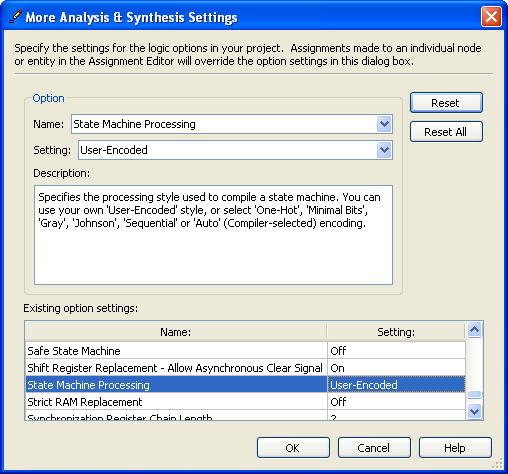
\includegraphics[scale = 0.75]{figures/figure4.png}}
\caption{Specifying the state assignment method in Quartus.}
\label{fig:fig7_4}
\end{figure}

\section*{Part III}
\addcontentsline{toc}{3}{Part III}
The sequence detector can be implemented in a straightforward manner using shift registers,
instead of using the more formal approach described above. Create Verilog code that
instantiates two 4-bit shift registers; one is for recognizing a sequence of four 0s, and
the other for four 1s. Include the appropriate logic expressions in your design
to produce the output $z$. Make a Quartus project for your design and implement
the circuit on your DE-series board. Use the switches and LEDs on the board in a similar way as
you did for Parts I and II and observe the behavior of your shift registers and the
output $z$. Answer the following question: could you use just one 4-bit shift
register, rather than two? Explain your answer.

~\newpage
\section*{Part IV}
\addcontentsline{toc}{4}{Part IV}
In this part of the exercise you are to implement a Morse-code encoder using an FSM. The Morse code uses
patterns of short and long pulses to represent a message. Each letter is represented as a sequence of dots
(a short pulse), and dashes (a long pulse). For example, the first eight letters of the alphabet have the
following representation:
~\\
\begin{center}
\begin{minipage}[t]{12.5 cm}
\begin{tabbing}
ZZ\=ZZ\=ZZ\=ZZ\=ZZ\=ZZ\=ZZ\=ZZ\=ZZ\=ZZ\=ZZ\kill
\>A\>\>{\bf $\bullet$  ---}\\
\>B\>\>{\bf ---  $\bullet$  $\bullet$  $\bullet$}\\
\>C\>\>{\bf ---  $\bullet$  ---  $\bullet$}\\
\>D\>\>{\bf ---  $\bullet$  $\bullet$}\\
\>E\>\>{\bf $\bullet$}\\
\>F\>\>{\bf $\bullet$  $\bullet$  ---  $\bullet$}\\
\>G\>\>{\bf ---  ---  $\bullet$}\\
\>H\>\>{\bf $\bullet$  $\bullet$  $\bullet$  $\bullet$}\\
\end{tabbing}
\end{minipage}
\end{center}

~\\
Design and implement a Morse-code encoder circuit using an FSM. Your circuit should take as input one of the first eight letters of the alphabet and display the Morse code for it on a red LED. Use switches {\it SW}$_{2-0}$ and pushbuttons {\it KEY}$_{1-0}$ as inputs. When a user presses {\it KEY}$_1$, the circuit should display the Morse code for a letter specified by {\it SW}$_{2-0}$ (000 for A, 001 for B, etc.), using 0.5-second pulses to represent dots, and 1.5-second pulses to represent dashes. Pushbutton {\it KEY}$_0$ should function as an asynchronous reset. 

A high-level schematic diagram of a possible circuit for the Morse-code encoder 
is shown in Figure~\ref{fig:morse_code_cct}.

\begin{figure} [H]
\begin{center}
	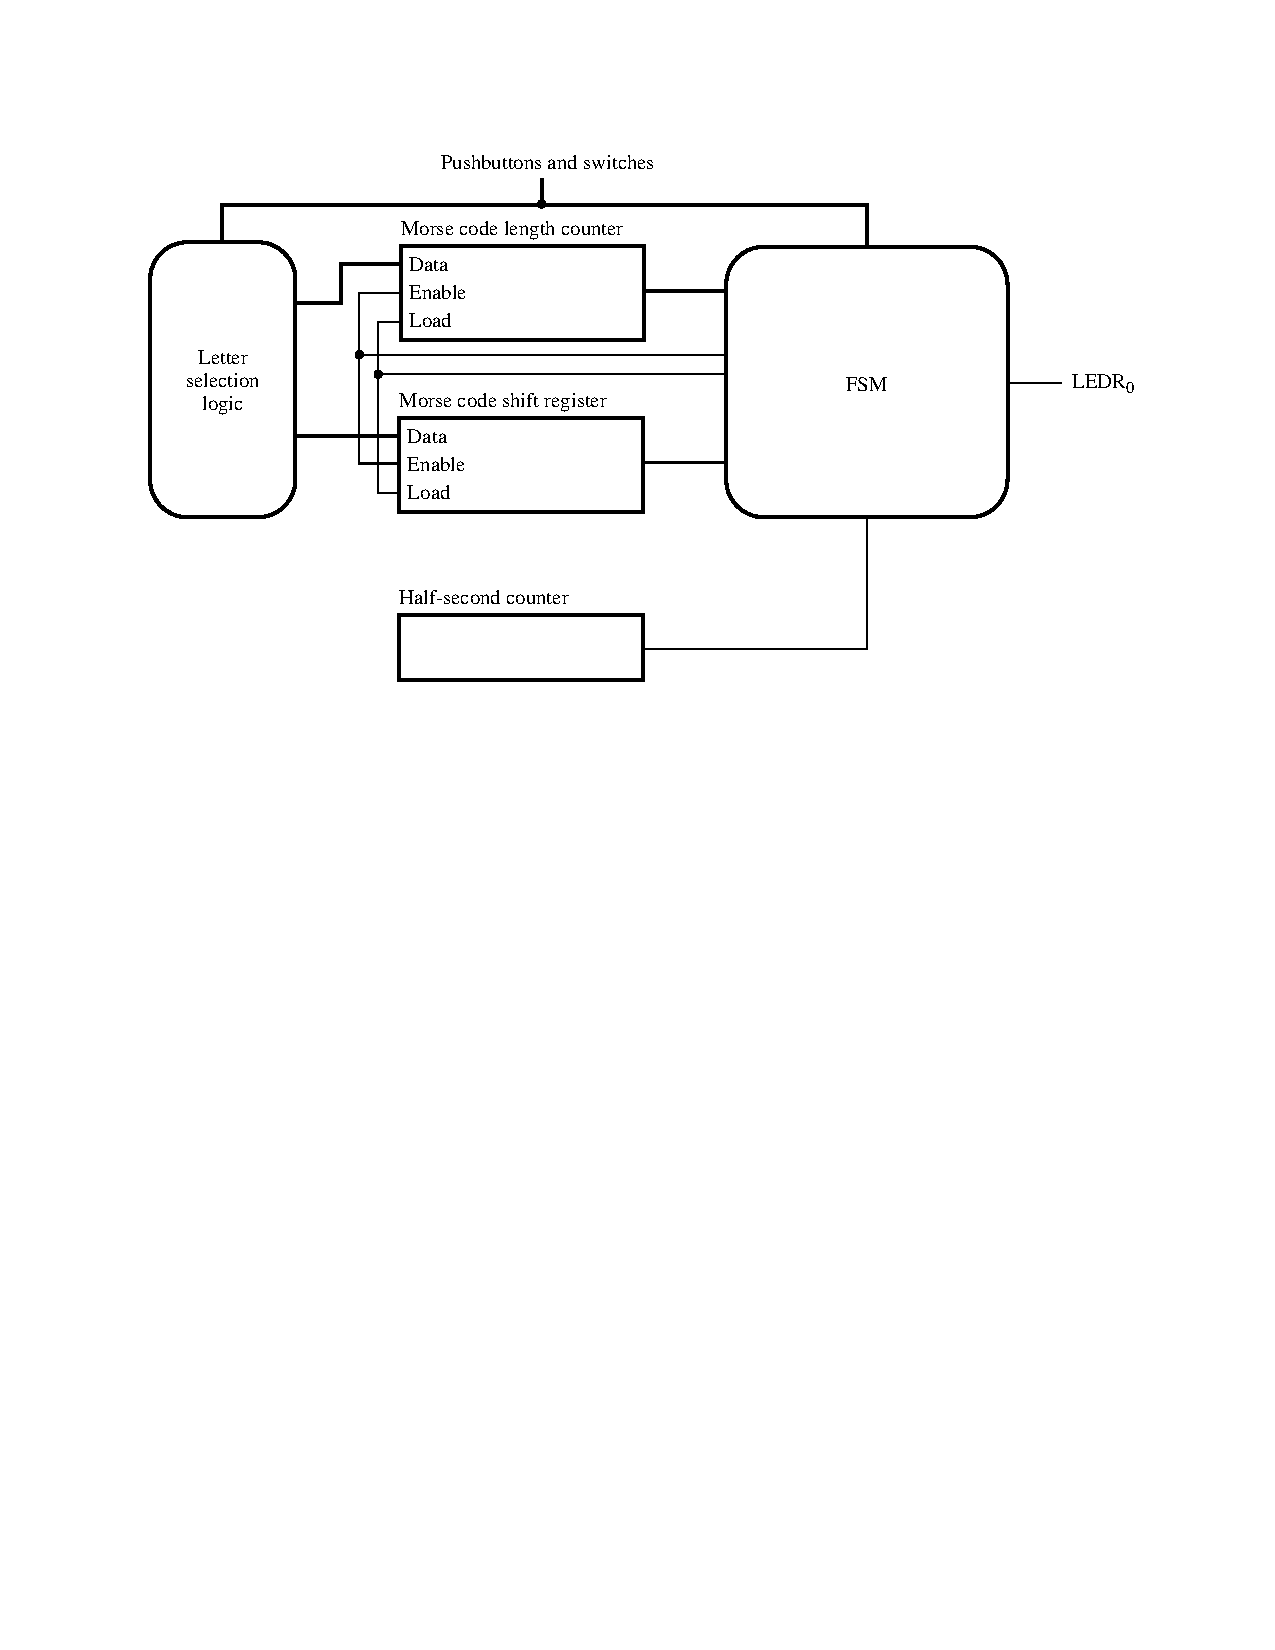
\includegraphics[scale = 0.9]{figures/fig_morse_code_circuit_schematic.pdf}
\end{center}
\caption{High-level schematic diagram of the circuit for Part IV.}
\label{fig:morse_code_cct}
\end{figure}


%%%%%%%%%%%%%%%%%%%%%%%%%%%%%%%%%%%%%%%%
%%% FPGAcademy Copyright Information %%%
%%%%%%%%%%%%%%%%%%%%%%%%%%%%%%%%%%%%%%%%

%Always put the copyright on a new page (clear page), with some vertical space from top
\clearpage
\vspace{1in}

\noindent

Copyright {\copyright} FPGAcademy.org. All rights reserved. FPGAcademy and the 
FPGAcademy logo are trademarks of FPGAcademy.org.  This document is provided 
"as is", without warranty of any kind, express or implied, including but not 
limited to the warranties of merchantability, fitness for a particular purpose 
and noninfringement. In no event shall the authors or copyright holders be 
liable for any claim, damages or other liability, whether in an action of 
contract, tort or otherwise, arising from, out of or in connection with the 
document or the use or other dealings in the document.
~\\
~\\
**Other names and brands may be claimed as the property of others.


\end{document}
